\documentclass[14pt,a4paper]{extarticle}
\usepackage[utf8]{inputenc}
\usepackage[T2A]{fontenc}
\usepackage[english,russian]{babel}
%\usepackage{fontspec}
%\setmainfont{Times New Roman} 
\usepackage[unicode]{hyperref}
\usepackage[left=2cm,right=1cm, top=2cm, bottom=2cm]{geometry}
\linespread{1.5}
\usepackage{indentfirst}
\usepackage{amssymb}
\usepackage{cmap}
\usepackage[]{graphicx}
\usepackage{hyperref}
\usepackage{array}
\usepackage{wrapfig}
\usepackage{longtable}
\usepackage{verbatim}
\usepackage{enumitem}
\usepackage{amsmath}
\usepackage{float}
\usepackage{mathtools}
\usepackage{icomma}
\usepackage{caption}
\captionsetup{labelsep=period}
\usepackage{xcolor}
\usepackage{animate}
%\numberwithin{equ`tion}{section}
\newcommand{\ten}[1]{\cdot 10^{#1}}
\hypersetup{
	colorlinks,
	citecolor=black,
	filecolor=black,
	linkcolor=black,
	urlcolor=blue
}

\usepackage{pdfpages}
\newcommand{\whr}{\text{, где}}
\newcommand{\razm}[1]{\hspace{1ex} \ensuremath{\left[\text{#1}\right]}}
\newcommand{\rbf}[1]{\textbf{\ref{#1}}}
\newcommand{\refris}[1]{рис. \rbf{#1}}
\newcommand{\prf}[1]{стр. \textbf{\pageref{#1}}}
\newenvironment{aleq}{\begin{equation}\begin{aligned}}{\end{aligned}\end{equation}}
\renewcommand{\geq}{\geqslant}
\renewcommand{\leq}{\leqslant}
\newcommand{\rt}[1]{_\text{#1}}
\newcommand{\mm}{\razm{мм}}

\renewcommand{\phi}{\varphi}
\renewcommand{\epsilon}{\varepsilon}

\newcommand{\an}[2]{a_{#1}\cos \left({#2}\frac{2\pi x}{P}\right)}
\newcommand{\bn}[2]{b_{#1}\sin \left({#2}\frac{2\pi x}{P}\right)}
\newcommand{\mtrig}[2]{\frac{2}{{#2}\pi}{#1}\left({#2}\frac{2\pi x}{P}\right)}
\author{Максим Зотов}
\title{МТ11-62Б}
\date{Вариант  5}
\begin{document}
\maketitle
\tableofcontents
\pagebreak
\section{Заданные условия}
\begin{center}
\begin{tabular}{lccc}
	Длина волны излучения &$\lambda$ & 0.24 &\razm{мкм}\\
	Апертура объектива &$A$ & 0.44 &\\
	Период решётки на фотошаблоне&$P$ & 1 &\razm{мкм}\\
	Ширина светлой полосы&$W$ & 0.5 &\razm{мкм}\\
	Профиль распределения интенсивности на объекте & & прямоугольный\\
\end{tabular}
\end{center}
\section{Краткое описание последовательности выполняемых этапов}
\begin{enumerate}
	\item Находим предельную частоту на единицу длины, пропускаемую объективом
	\begin{equation}
		\nu_{\lim} = \frac{2 A P }{\lambda} = \frac{2\cdot 0.44}{0.24} = 3.667 \approx 3\razm{$\frac{1}{\text{мм}}$} 
	\end{equation}
	\item Находим значения частот в относительных едицах
	\begin{equation}
		R = \frac{\nu}{\nu_{\lim}} =  \frac{\nu}{P}\cdot\frac{\lambda}{2A}, \quad \nu =  
		\begin{pmatrix}
			0\\
			1\\
			2\\
			3\\
		\end{pmatrix}, \quad R = 
		\begin{pmatrix}
			0\\
			0.273\\
			0.545\\
			0.818\\
		\end{pmatrix}
	\end{equation}
	\item Находим значения функции передачи модуляции
	\begin{equation}
		T(\nu) = \frac{2}{\pi} \left(\arccos (R) - R\sqrt{1-R^2}\right), \quad R = 
		\begin{pmatrix}
			0\\
			0.273\\
			0.545\\
			0.818\\
		\end{pmatrix}, \quad T = 
		\begin{pmatrix}
			1\\
			0.657\\
			0.342\\
			0.09\\
		\end{pmatrix}
	\end{equation}
	\item 
\end{enumerate}

\section{Математическое обеспечение основных этапов}
\subsection{Разложение функции  по Фурье}
Периодическую функцию $f(x)$, имеющую период $P$, т. е. пространственную частоту $\nu = \frac{1}{P}$, можно представить в виде суммы синусоид или косинусоид, имеющих частоты $\nu $, $2\nu$, $3\nu$ \ldots $n\nu$ \razm{$\frac{1}{\text{мм}}$}  и периоды $P$, $\frac{P}{2}$, $\frac{P}{2}$, \ldots, $\frac{P}{n}$ \razm{мм}:
\begin{multline}
	f(x) = \frac{a_0}{2} + \an{1}{} + \bn{1}{} + \ldots + \an{n}{n} + \bn{n}{n}= \\
	= \frac{a_0}{2} + \sum \limits _ {n = 1} ^ {\infty} \an{n}{n} + \sum \limits _ {n = 1} ^ {\infty} \bn{n}{n}
\end{multline}

Коэффициенты такого ряда определяются по формулам
\begin{aleq}
	a_0& = \frac{2}{P} \int \limits _{P} f(x) dx \\
	a_n& = \frac{2}{P} \int \limits _{P} f(x) \cos \left(\frac{2\pi n x}{P}\right) dx \\
	b_n& = \frac{2}{P} \int \limits _{P} f(x) \sin \left(\frac{2\pi n x}{P}\right) dx
\end{aleq}

Решетки с одинаковыми прозрачными и непрозрачными полосами, могут быть описаны рядами Фурье (расположим начало координат на границе окна)
\begin{equation}
	f(x) = 0.5 + \mtrig{\sin}{} + \mtrig{\sin}{3} + \mtrig{\sin}{5}
\end{equation}
\subsection{Учет распределения интенсивности в изображении}
\begin{enumerate}
	\item Для известного (заданного) пространственного распределения интенсивности $I_0(x)$ в объекте находят частотное распределение объекта  $I_0(\nu)$ с помощью Фурье - преобразования:
	\begin{equation}
		I_0(\nu) = F_T [I_0(x)]
	\end{equation}
	\item Предварительно для каждой пропускаемой частоты рассчитывают соответствующее значение $T(\nu)$ коэффициента передачи модуляции, далее умножают его на значение коэффициента Фурье соответствующей гармоники.:
	\begin{equation}
		I_i(\nu) = T(\nu)[I_0(\nu)]
	\end{equation}

	\item Находят пространственное распределение интенсивности в изображении за счет обратного фурье-преобразования:
	\begin{equation}
		I_i(x) = F_T^{-1} [I_i(\nu)]
	\end{equation}
	\item Оценивают распределение интенсивности в изображении с технологической точки зрения. Дифракционное размытие изображения приводит к тому, что на участки фоторезиста, лежащие в области геометрической тени, попадает часть экспонирующего излучения. Получаемая этими участками доза экспозиции может стать достаточной для утонения фоторезиста, в результате он не сможет служить защитной маской при последующих операциях.
\end{enumerate}
\subsection{Оценка применимости литографической системы}
Для количественной оценки качества пространственного изображения в оптике используют
понятие \textit{модуляции}, т. е. отношения амплитуды распределения интенсивности $I_a$ к среднему
значению $I_m$. Часто применяется также \textit{эквивалентное }понятие контраста, который
выражается через максимальное $I_{\max}$ и минимальное $I_{\min}$ значения интенсивности (освещенности)
изображения:
\begin{equation}\label{eq:contrast}
	T = \frac{I_a}{I_m} = \frac{I_{\max}-I_{\min}}{I_{\max}+I_{\min}}
\end{equation}

Для получения микрорельефа в фоторезисте необходимо, чтобы модуляция оптического изображения превышала модуляцию фоторезиста, таким образом, на значение оптического контраста наклыдывается ограничение
\begin{equation}\label{eq:Tmin}
	T\geq 0.6
\end{equation}

Получив значения $I_{\max}$ и $I_{\min}$ при помощи Matlab (см \refris{gr:ob}) и подставив их в \eqref{eq:contrast} и \eqref{eq:Tmin} получим
\begin{multline}
	 T = \frac{I_{\max}-I_{\min}}{I_{\max}+I_{\min}} = \frac{0.899 - 0.101}{0.899 + 0.101} \approx 0.798 > 0.6\\ \text{\hspace{3mm}(проведение фотолитографии возможно})
\end{multline}
\section{Программное обеспечение}
Приведённый ниже код работает с большинством возможных значений апертуры, периода и длины волны. Сначала вычисляется количество элементов в матрице $R$. Затем находятся значения $T(\nu)$. После этого строится исходное распределение, его представление в виде Фурье - разложения, график Фурье - разложения после объектива и график функции передачи модуляции.
 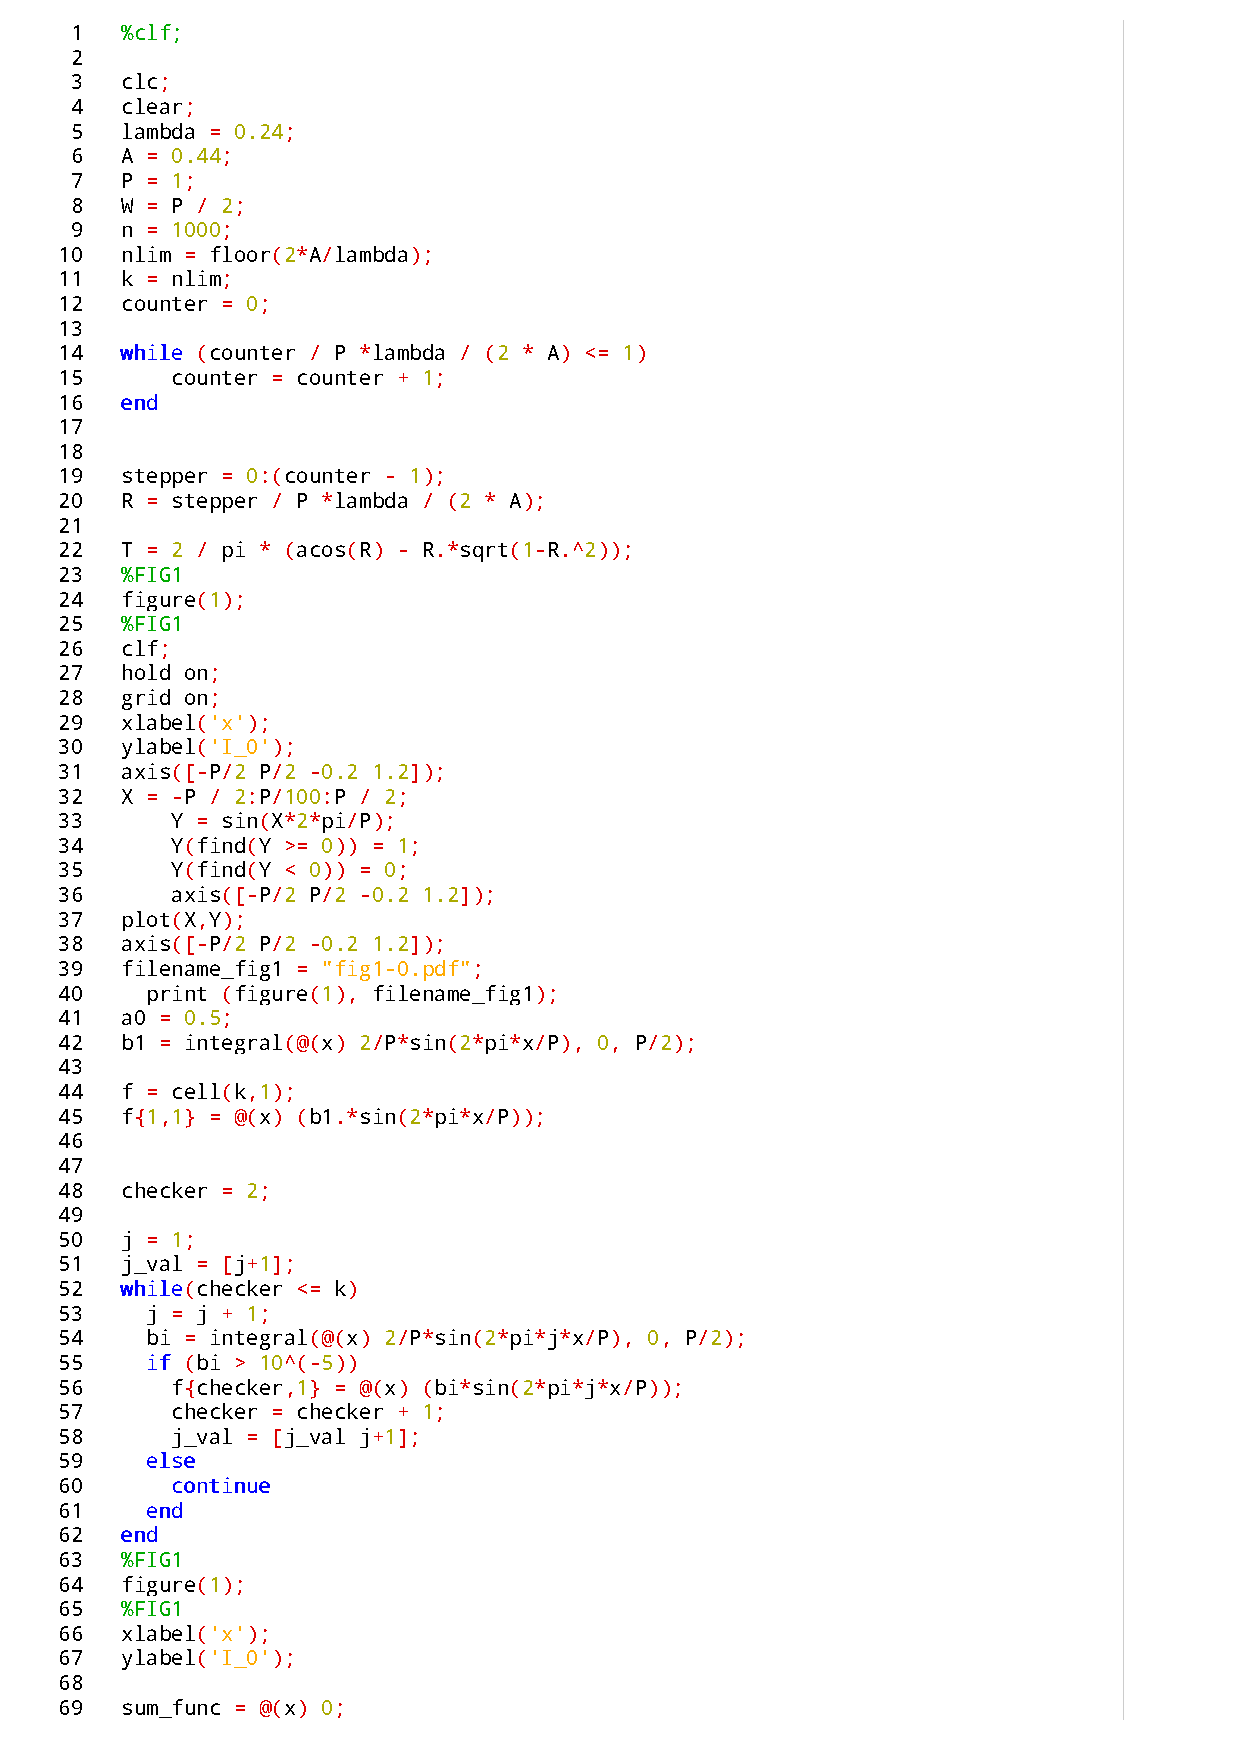
\includepdf[pages=-]{print.pdf} 
\section{Графики}
\subsection{Входное распределение интенсивности (на объекте)}
\begin{figure}[H]\caption{Входное распределение интенсивности}\label{gr:vhod}
	\centering
	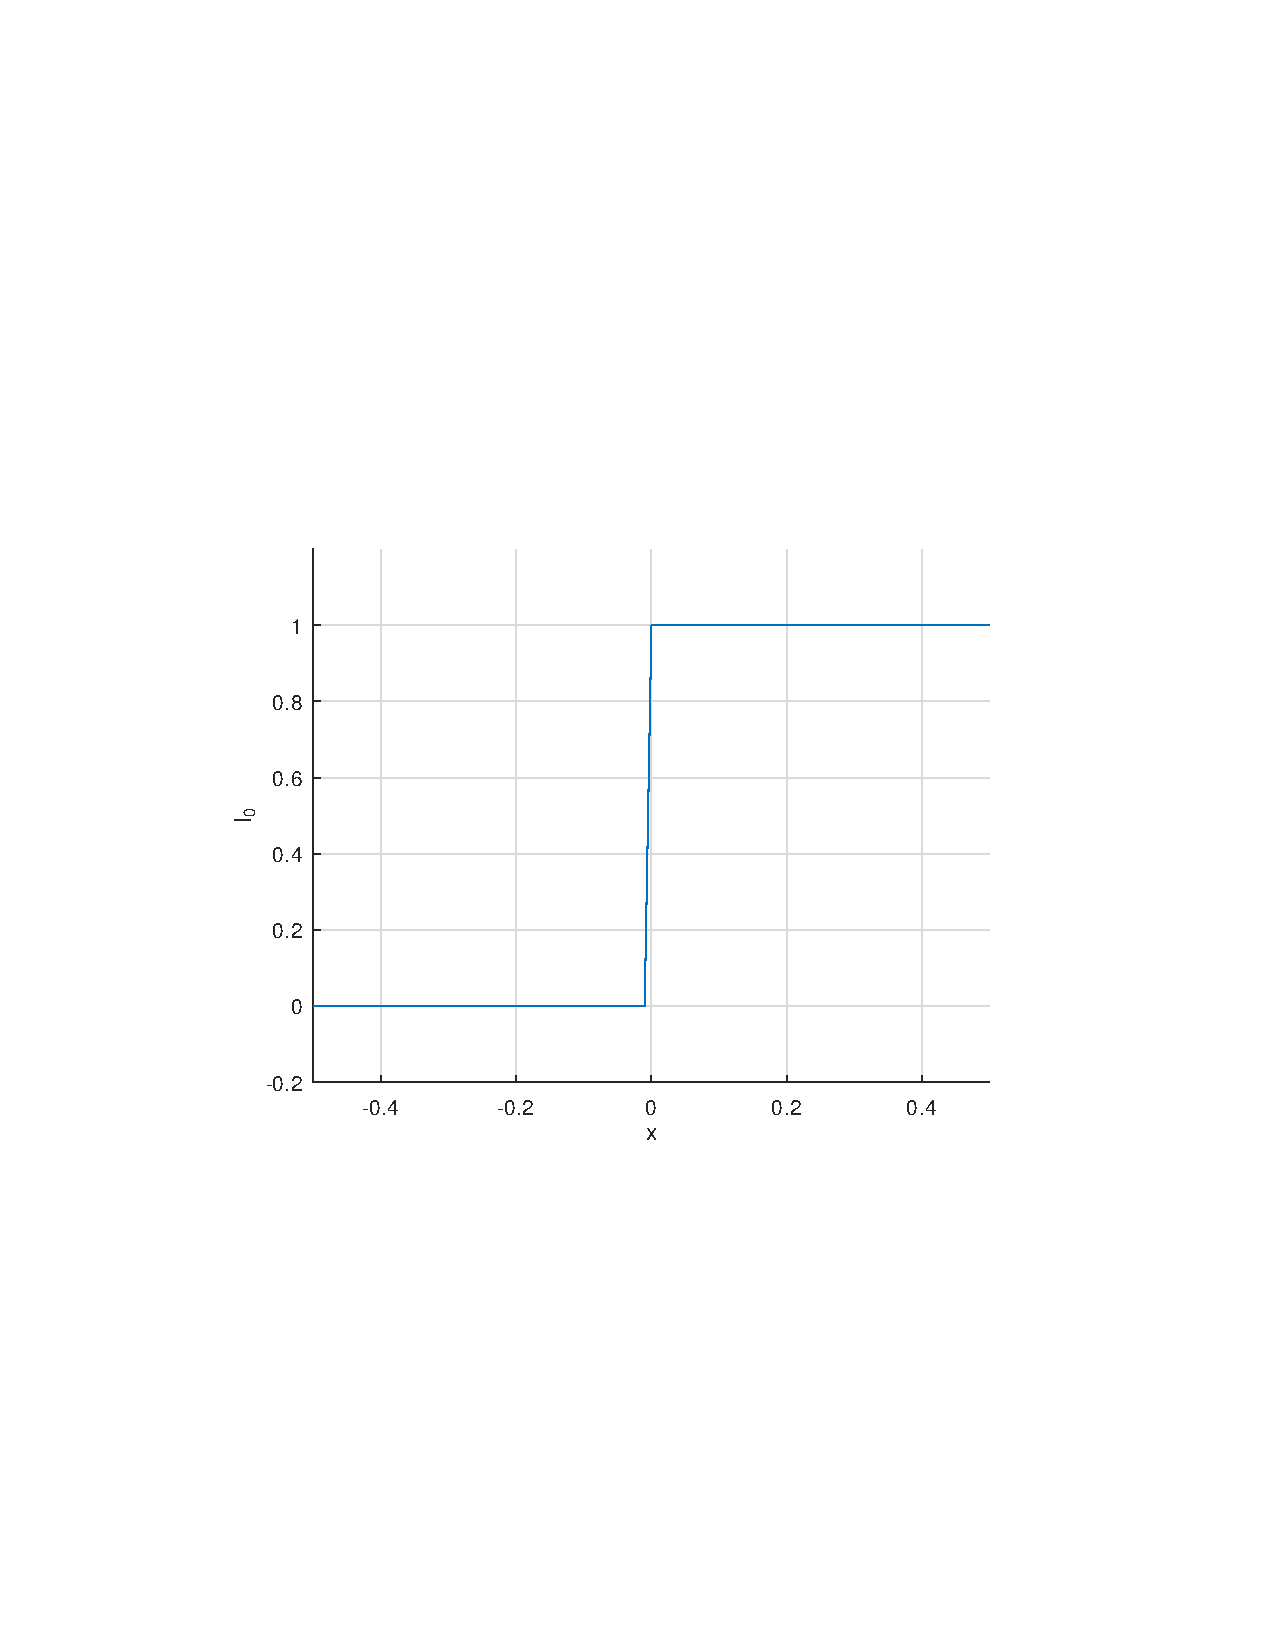
\includegraphics[trim=110 230 110 290,clip, width=0.6\textwidth]{fig1-0.pdf}
\end{figure}
\subsection{Представления входного распределения Фурье - разложением}
\begin{figure}[H]
	\begin{center}\caption{Представление входной интенсивности Фурье - разложением (анимация по гармоникам)}\label{gr:fourier}
		\animategraphics[trim=110 230 110 270, loop,controls={play,step},width=0.6\textwidth]{1}{fig1-}{0}{4}
	\end{center}
\end{figure}

\subsection{Фурье - разложения после объектива}
\begin{figure}[H]
	\begin{center}\caption{Фурье - разложения после объектива}\label{gr:ob}
		\animategraphics[trim=110 230 110 260, loop,controls={play,step},width=0.6\textwidth]{1}{fig2-}{1}{3}
	\end{center}
\end{figure}
\subsection{Суммарный профиль распределения интенсивности в плоскости изображения}
\begin{figure}[H]
	\begin{center}\caption{Суммарный профиль распределения интенсивности в плоскости изображения}\label{gr:kpm}
		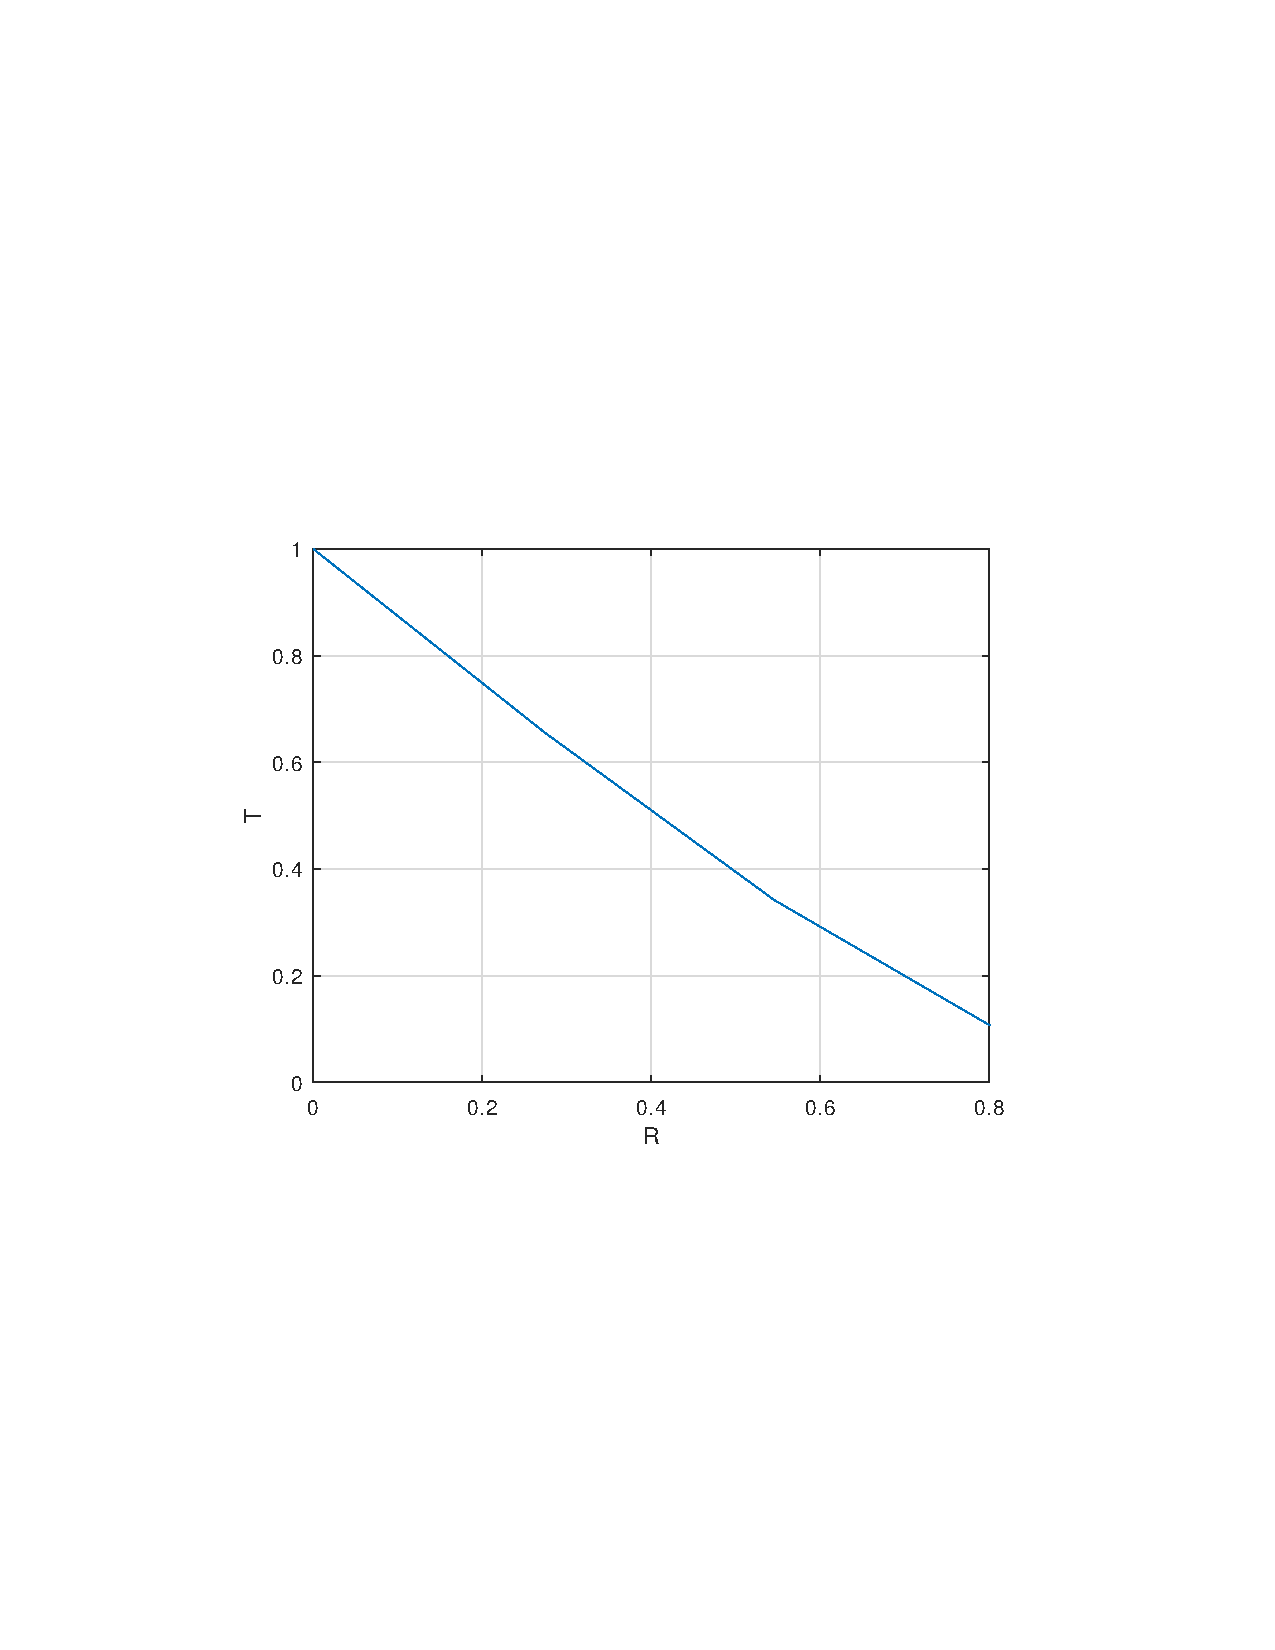
\includegraphics[trim=110 230 110 250,clip, width=0.5\textwidth]{fpm.pdf}
	\end{center}
\end{figure}
\end{document}